
\subsection{Description of DNA Mismatch Repair}

We now return to the DNA mismatch repair, which we have briefly described in the introduction, and we give a fuller explanation of how it works.
%Such a repair is not possible in the same way as the base excision repair (BER), since any of the two bases could be wrong, so the non-matching  bases do not tell what to do. In contrast, to repair the incorporation of a uracil, clearly the uracil must be removed and replaced. A description of the process on an abstract level is as follows:
If two bases are incorporated into a DNA strand which do not match, namely are not A-T or C-G pairs, this constitutes a defect in the DNA strand. A repair similar to BER is not possible, since it is not clear which of the two bases is correct.
% just from the bases alone - both could be right.
We are looking at a specific way to handle this situation, called Methyl Mismatch Repair (MMR). This is the repair mechanism in bacteria, in particular E.\! coli, for which detailed studies has been done\footnote{Paul L. Modrich, Tomas Lindahl and Aziz Sancar received the Nobel Price in Chemistry 2015 for their work on DNA repair. Modrich's Nobel Lecture about Methyl-directed Mismatch Repair in E. coli and humans \cite{pmid27198632} gives a good overview.}.
The mechanism relies on DNA strands being methylated sometime after their creation. Methylation means the attachment a methyl group (a carbon atom with three hydrogen atoms), in this case to the adenine base A. Specifically, this happens whenever there is a GATC sequence. Since the methylation %(which is done by specific proteins, which we do not model)
happens with a delay after the duplication of a strand, old strand is methylated and the new strand is not methylated for a short period of time. This enables the removal of the wrong base from the new strand.

The actual repair involves the proteins MutS, MutL, MutH, and UvrD. MutS first binds to the mismatch and then recruits MutL and MutH. MutL can detect the methylated strand and can form a loop in the DNA. In this loop, the newer strand is now outside, whereas the old strand is covered by itself and MutL. Then MutH cleaves the unmethylated strand. This happens in some distance from the mismatch, due to the size of the proteins and the loop in the DNA. UvrD can then detect the cleavage and can move along the strand towards the site of the mismatch. It removes the outer strand when moving along. At the same time, the MutL, MutH, and MutS proteins are released and the loop in the DNA disappears. Finally UvrD moves to a position immediately beyond the mismatch, removing the wrong base together with its neighbours. UvrD then goes off the DNA and leaves the old, and correct, strand to be completed.

\subsection{DNA Mismatch Repair System}

Having briefly introduced all major components that are involved in this mismatch repair mechanism, we now
define them in the syntax of CCB. Our intention is to reuse the components from \cite{10.1007/978-3-319-99498-7_8} as much as possible. Specifically, we reuse the deoxyribose/phosphate groups, and the four bases A, T, C, and G. We will extend those components where needed, but we will keep the original actions. We need the following components for the MMR system: deoxyribose/phosphate groups (DP), the four bases A, T, G, C, the methyl group Me, and the proteins MutS, MutL, MutH, and UvrD. The reused components are as follows:
%
$$\begin{array}{lll}
\DP & \bydef & ((p3,p5;s) \paral (b,d)).\DP'\\
A & \bydef & (b;i).(a,m;r).A'\\
T & \bydef & (b;i).(t;r).T'\\
G & \bydef & (b;i).(g;r).G'\\
C & \bydef & (b;i).(c;r).C'\\
\end{array}$$
%
%where processes $A$, $T$, $G$, and $C$ model the bases adenine (A), cytosine (C), guanine (G), and thymine (T).
Notice that we have added new actions $s$, $m$, and $r$. The action $m$ enables the methylation. It only exists in $A$ since the methylation happens only there. %Also, the actions on DP have been regrouped (but all original actions are still there).
In $\DP$, we now use a collection with two sites. This is necessary to enable breaking of a bond to $p3$ or $p5$, which are on one site, whilst there is still a bond to $b$ on the other site. %The action $d$, which was used by UDG in the modelling of BER is not used here, as we will see. We keep it to have an extension of the previous modelling.

We also need additional components, namely the methyl group Me, and the MutS, MutL, MutH, and UvrD proteins. They are defined as follows:
$$\begin{array}{lll}
\Me & \bydef & (m).(n).\Me' \\
\MutS & \bydef & (k,k).(l).\MutS'\\
\MutL & \bydef & (l).(n).(o).\MutL'\\
\MutH & \bydef & (o).(w).\MutH'\\
\UvrD & \bydef & ((u;r) \paral (v;s)).\UvrD'\\
\end{array}$$
%
%where processes $MutS$, $MutL$, $MutH$, and $UvrD$ model the MutS, MutL, MutH, and UvrD protein respectively.
Here $s$, $i$, and $r$ are weak actions, all other actions, namely $p3$, $p5$, $b$, $d$, $a$, $t$, $g$, $c$, $m$, $n$, $k$, $l$, $o$, $s$, $u$, $v$ and $w$, are strong. Notice that $i$ is not used here, but we keep it to have this model as an extension of the BER model~\cite{10.1007/978-3-319-99498-7_8}. In $\UvrD$, we again use a prefix with two sites.
This will make it possible for $\UvrD$ to break two bonds (one from each site) as it ``moves'' along a DNA strand.


The synchronisation function for our system is as follows:
%
\[\arraycolsep=3.4pt\def\arraystretch{1.0}
\begin{array}{ l c l | l c l | l c l | l c l}
\gamma(p3,p5) & = & p & \gamma(b,b) & = & bb & \gamma(a,t) & = & at &  \gamma(g,c) & = & gc \\
\hline
\gamma(m,m) & = & mm & \gamma(k,a) & = & ka & \gamma(k, g) & = & kg & \gamma(k,c) & = & kc \\
\hline
\gamma(k,t) & = & kt & \gamma(l,l) & = & ll &\gamma(n,n) & = & nn & \gamma(o,o) & = & oo\\
\hline
\gamma(r,r) & = & rr & \gamma(t,u) & = & tu &\gamma(p,s) & = & ps &\gamma(w,s) & = & ws\\
\hline
\gamma(s,p3) & = & sp3 &  \gamma(v,p3) & = & vp3 &\gamma(w,p3) & = & wp3  & \gamma(u,r) & = & ur \\
\hline
\gamma(s,s) & = & ss & \gamma(s,v) & = & sv & \gamma(u,c) &=  & uc &  \\
\end{array}
\]
The deoxyribose/phosphate groups and the bases can combine to form a DNA strand. There can be DNA mismatches in such strands. Note that we do not model how they happen, we just assume a DNA strand as in Figure~\ref{fig:state1} with one DNA mismatch. % and correct pairs otherwise.
The mismatch here is on the $A_2$ and $G_3$ pair.
%, but that is not crucial for our modelling.
The A and G bases cannot bond to each other--it is the case in our model as well as in reality--and this gives the opportunity for the repair. There is a CTAG sequence (respectively a GATC sequence) on the top left (respectively bottom left)
chain of the DNA in Figure~\ref{fig:state1}. This is where the methylation happens. In our case, we have a recently duplicated strand, where the older chain is the upper one ($A_1$ is methylated there) and the newer chain is the lower one (where A is not methylated). The methylation is done by proteins which are not modelled here.
%This is the situation where the MMR can happen.

\begin{figure}[h!]
\psfrag{dp1}{$DP_1$}
\psfrag{dp2}{$DP_2$}
\psfrag{dp3}{$DP_3$}
\psfrag{dp4}{$DP_4$}
\psfrag{dp5}{$DP_5$}
\psfrag{dp6}{$DP_6$}
\psfrag{dp7}{$DP_7$}
\psfrag{dp8}{$DP_8$}
\psfrag{dp9}{$DP_9$}
\psfrag{dp10}{$DP_{10}$}
\psfrag{dp11}{$DP_{11}$}
\psfrag{dp12}{$DP_{12}$}
%\psfrag{A1}[cc][][0.8][0]{{$\mathit{A_1}}$}
\psfrag{A1}[cc][][0.8][0]{$A_1$}
\psfrag{A2}[cc][][0.8][0]{$A_2$}
\psfrag{A3}[cc][][0.8][0]{$A_3$}
\psfrag{T1}[cc][][0.8][0]{$T_1$}
\psfrag{T2}[cc][][0.8][0]{$T_2$}
\psfrag{C1}[cc][][0.8][0]{$C_1$}
\psfrag{C2}[cc][][0.8][0]{$C_2$}
\psfrag{C3}[cc][][0.8][0]{$C_3$}
\psfrag{G1}[cc][][0.8][0]{$G_1$}
\psfrag{G2}[cc][][0.8][0]{$G_2$}
\psfrag{G3}[cc][][0.8][0]{$G_3$}
\psfrag{G4}[cc][][0.8][0]{$G_4$}
\psfrag{Me}{${\mathit{Me}}$}
\psfrag{MS}{${\mathit{MutS}}$}
\psfrag{ML}{${\mathit{MutL}}$}
\psfrag{MH}{${\mathit{MutH}}$}
\psfrag{UD}{${\mathit{UvrD}}$}
  \centering
    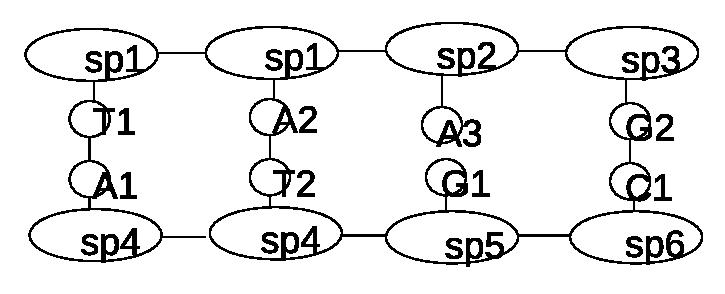
\includegraphics[width=1.0\textwidth]{mmr/state1}
  \caption[A six base pair DNA fragment.]{A six base pair DNA fragment, with a DNA mismatch and methylation of an upper strand. The proteins MutL, MutS, MutH, and UvrD are currently not bonded to the DNA.}
  \label{fig:state1}
\end{figure}

The system shown in Figure~\ref{fig:state1} is modelled in CCB as follows:
%We can model this similar to what we did before as:

$$\begin{array}{l}
(\DP_1 \paral \DP_2 \paral \DP_3 \paral \DP_4 \paral \DP_5 \paral \DP_6 \paral \\
C_1 \paral T_1 \paral A_1 \paral G_1 \paral A_2 \paral C_2 \paral \\
G_2 \paral A_3 \paral T_2 \paral C_3 \paral G_3 \paral G_4 \paral \\
\DP_7 \paral \DP_8 \paral \DP_9 \paral \DP_{10} \paral \DP_{11} \paral \DP_{12} \paral \\
\Me \paral \MutS \paral \MutL \paral \MutH \paral \UvrD) \\
\setminus\{p3, p5, s, i, r, b, b, d, b, a, t, g, c, m, n, k, l, o, s, u, v, w\}
\end{array}$$

We leave out the restriction from now on for ease of reading. We mark copies of processes $\DP$ and the bases, and their actions, using subscripts in order to make them unique. Pairs of keys show on which actions the initial bonds have been created. The MMR  system in full detail (but without restriction) is given below.
%
\begin{flalign*}
&((p3_1,p5_1[1];s_1) \paral (b_1[10],d_1)).DP_1' \paral ((p3_2[1],p5_2[2];s_2) \paral (b_2[8],d_2)).DP_2' \paral &&\\
&((p3_3[2],p5_3[3];s_3) \paral (b_3[6],d_3)).DP_3' \paral ((p3_4[3],p5_4[4];s_4) \paral (b_4[9],d_4)).DP_4' \paral &&\\
&((p3_5[4],p5_5[5];s_5) \paral (b_5[7],d_5)).DP_5' \paral ((p3_6[5],p5_6;s_6) \paral (b_6[11],d_6)).DP_6' \paral  &&\\
&(b_{10}[10];i_{10}).(c_1[41];r_{10}).C_1' \paral (b_4[8];i_4).(t_1[23]:r_4).T_1' \paral (b_1[6];i_1).(a_1[24],m_1[40];r_1).A_1' \paral &&\\
& (b_6[9];i_6).(g_1[25];r_6).G_1' \paral (b_2[7];i_2).(a_2,m_2;r_2).A_2' \paral (b_{11}[11];i_{11}).(c_2[27];r_{11}).C_2' \paral &&\\
&(b_7[17];i_7).(g_2[41];r_7).G_2' \paral (b_3[18];i_3).(a_3[23],m_3;r_3).A_3' \paral (b_5[19];i_5).(t_2[24];r_5).T_2' \paral   &&\\
& (b_{12}[20];i_{12}).(c_3[25];r_{12}).C_3'  \paral (b_8[21];i_8).(g_3;r_8).G_3' \paral (b_9[22];i_9).(g_4[27];r_9).G_4' \paral&&\\
&((p3_7,p5_7[12];s_7) \paral (b_7[17],d_7)).DP_7' \paral ((p3_8[12],p5_8[13];s_8) \paral (b_8[18],d_8)).DP_8' \paral &&\\
&((p3_9[13],p5_9[14];s_9) \paral (b_9[19],d_9)).DP_9' \paral ((p3_{10}[14],p5_{10}[15];s_{10}) \paral (b_{10}[20],d_{10})).DP_{10}' \paral  &&\\
&((p3_{11}[15],p5_{11}[16];s_{11}) \paral (b_{11}[21],d_{11})).DP_{11}' \paral ((p3_{12}[16],p5_{12};s_{12}) \paral (b_{12}[22],d_{12})).DP_{12}' \paral  &&\\
&(m[40]).(n).Me'\paral (k,k).(l).MutS' \paral (l).(n).(o).MutL' \paral &&\\
&(o).(w).MutH' \paral (u;r) \paral (v;s).UvrD'&&
\end{flalign*}
$\DP_1$ is connected to $\DP_2$ via the bond on $p5_1$ and $p3_2$ with the key 1. Similarly, $\DP_1$ is bonded to $C_1$ via the bond on actions $b$ with the key 10. Also, $\Me$ is bonded with $A_1$ on $m$ with the key 40. Correspondingly, there are other initial bonds with appropriate keys in the MMR system as shown in Figure~\ref{fig:state1}. \textcolor{red}{It should be noted that the two processes above show the same system, and so does Figure~\ref{fig:state1}. The two notations above show different levels of detail, with the first only giving the process names and the second their definitions. Figure~\ref{fig:state1} shows the same level of detail as the second process. We do not say how this state emerged and how the bonds were formed.}


A mismatch in the DNA section in Figure~\ref{fig:state1} is between $A_2$ and $G_3$.
%: they do not form an A-T or G-C pair as required.
Methylation is on the old upper half of the strand, which means that a methyl group $\Me$ is attached to $A_1$. Note that there is no methyl group on $A_2$. This is because the methylation only happens on CTAG sequences via a specific protein, which we do not model here. %, we just assume the end result.
No bases $A$ are methylated on the new lower half, even if they parts of CTAG sequences, since not enough time has passed at this stage for this to happen.

Before we show the main reactions of the MMR mechanism, we shall shorten the presentation of our MMR system so that the reactions are more easily readable and can be quickly checked.  Since $\DP_1$, $\DP_2$, $\DP_3$, $\DP_4$, $\DP_5$, $\DP_6$, and $\DP_7$, and the bases $C_1$,  $T_1$, $C_2$, $G_2$, $A_3$, and $G_4$  (read from top to bottom and from left to right in Figure~\ref{fig:state1}) never directly participate in the reactions, we will leave them out from now on. The remaining part of the syntax of the MMR system is much smaller:
%
\begin{flalign*}
& (b_1[6];i_1).(a_1[24],m_1[40];r_1).A_1' \paral
(b_6[9];i_6).(g_1[25];r_6).G_1' \paral (b_2[7];i_2).(a_2,m_2;r_2).A_2' \paral  &&\\
& (b_5[19];i_5).(t_2[24];r_5).T_2' \paral
(b_{12}[20];i_{12}).(c_3[25];r_{12}).C_3'  \paral (b_8[21];i_8).(g_3;r_8).G_3' \paral &&\\
&  ((p3_8[12],p5_8[13];s_8) \paral (b_8[18],d_8)).\DP_8' \paral &&\\
&((p3_9[13],p5_9[14];s_9) \paral (b_9[19],d_9)).\DP_9' \paral ((p3_{10}[14],p5_{10}[15];s_{10}) \paral (b_{10}[20],d_{10})).\DP_{10}' \paral  &&\\
&((p3_{11}[15],p5_{11}[16];s_{11}) \paral (b_{11}[21],d_{11})).\DP_{11}' \paral ((p3_{12}[16],p5_{12};s_{12}) \paral (b_{12}[22],d_{12})).\DP_{12}' \paral  &&\\
&(m[40]).(n).\Me'\paral (k,k).(l).\MutS' \paral (l).(n).(o).\MutL' \paral &&\\
&(o).(w).\MutH' \paral (u;r) \paral (v;s).\UvrD'&&
\end{flalign*}
Note that leaving out some components results in appearance of  several ``incomplete'' bonds, for example, between
$\DP_8$ and $\DP_7$, which is left out, with the key 12.

\subsection{Reactions in DNA Mismatch Repair}


We now present the main reactions of the MMR system, thus illustrating the benefits of concerted actions transitions.

 We start with the protein $\MutS$ bonding to processes $A_2$ and $G_3$  via the $a_2$ and $g_3$ actions respectively. This is the recognition of the mismatch.
%Note that the $a$ and $g$ actions are not available on matching pairs. So the bonding is not possible if the bases are properly paired, and also not if a Uracil is incorporated into the strand (as in the BER example).
The transitions for creating the two bonds of $\MutS$ with
$A_2$ and $G_3$ are as follows, where first we highlight the participating actions in bold blue font and then we
highlight the actions and keys in bold black font after the bonds are created:

\begin{flalign*}
& (b_1[6];i_1).(a_1[24],m_1[40];r_1).A_1' \paral
(b_6[9];i_6).(g_1[25];r_6).G_1' \paral & & \\
& (b_2[7];i_2).(\Blue{\bm{a_2}},m_2;r_2).A_2' \paral  (b_5[19];i_5).(t_2[24];r_5).T_2' \paral
(b_{12}[20];i_{12}).(c_3[25];r_{12}).C_3'  \paral & & \\
& (b_8[21];i_8).(\Blue{\bm{g_3}};r_8).G_3' \paral  ((p3_8[12],p5_8[13];s_8) \paral (b_8[18],d_8)).\DP_8' \paral &&\\
&((p3_9[13],p5_9[14];s_9) \paral (b_9[19],d_9)).\DP_9' \paral ((p3_{10}[14],p5_{10}[15];s_{10}) \paral (b_{10}[20],d_{10})).\DP_{10}' \paral  &&\\
&((p3_{11}[15],p5_{11}[16];s_{11}) \paral (b_{11}[21],d_{11})).\DP_{11}' \paral ((p3_{12}[16],p5_{12};s_{12}) \paral (b_{12}[22],d_{12})).\DP_{12}' \paral  &&\\
&(m[40]).(n).\Me'\paral (\Blue{\bm{k}},\Blue{\bm{k}}).(l).\MutS' \paral (l).(n).(o).\MutL' \paral &&\\
&(o).(w).\MutH' \paral (u;r) \paral (v;s).\UvrD'&&\\
%
&\xrightarrow{ka[28]} \xrightarrow{kg[29]} &&\\
%
& (b_1[6];i_1).(a_1[24],m_1[40];r_1).A_1' \paral (b_6[9];i_6).(g_1[25];r_6).G_1' \paral &&\\
&(b_2[7];i_2).(\bm{a_2[28]},m_2;r_2).A_2' \paral  (b_5[19];i_5).(t_2[24];r_5).T_2' \paral (b_{12}[20];i_{12}).(c_3[25];r_{12}).C_3'  \paral &&\\
&(b_8[21];i_8).(\bm{g_3[29]};r_8).G_3' \paral ((p3_8[12],p5_8[13];s_8) \paral (b_8[18],d_8)).\DP_8' \paral &&\\
&((p3_9[13],p5_9[14];s_9) \paral (b_9[19],d_9)).\DP_9' \paral ((p3_{10}[14],p5_{10}[15];s_{10}) \paral (b_{10}[20],d_{10})).\DP_{10}' \paral &&\\
&((p3_{11}[15],p5_{11}[16];s_{11}) \paral (b_{11}[21],d_{11})).\DP_{11}' \paral ((p3_{12}[16],p5_{12};s_{12}) \paral (b_{12}[22],d_{12})).\DP_{12}' \paral  &&\\
&(m[40]).(n).\Me'\paral (\bm{k[28],k[29]}).(\Blue{\bm{l}}).\MutS' \paral (\Blue{\bm{l}}).(n).(o).\MutL' \paral &&\\
&(o).(w).\MutH' \paral ((u;r) \paral (v;s)).\UvrD'&&
\end{flalign*}

Now it is possible for $\MutL$ to bond to $\MutS$ on $l$ with key 30 (see Figure~\ref{fig:state15}). Again, the participating actions $l$ are in bold blue font before the transition and then they are displayed in bold black font:
%
\begin{flalign*}
&\xrightarrow{ll[30]} (b_1[6];i_1).(a_1[24],m_1[40];r_1).A_1' \paral (b_6[9];i_6).(g_1[25];r_6).G_1' \paral &&\\
&(b_2[7];i_2).(a_2[28],m_2;r_2).A_2' \paral (b_5[19];i_5).(t_2[24];r_5).T_2' \paral  (b_{12}[20];i_{12}).(c_3[25];r_{12}).C_3'  \paral &&\\
&(b_8[21];i_8).(g_3[29];r_8).G_3' \paral ((p3_8[12],p5_8[13];s_8) \paral (b_8[18],d_8)).\DP_8' \paral &&\\
&((p3_9[13],p5_9[14];s_9) \paral (b_9[19],d_9)).\DP_9' \paral ((p3_{10}[14],p5_{10}[15];s_{10}) \paral (b_{10}[20],d_{10})).\DP_{10}' \paral  &&\\
&((p3_{11}[15],p5_{11}[16];s_{11}) \paral (b_{11}[21],d_{11})).\DP_{11}' \paral ((p3_{12}[16],p5_{12};s_{12}) \paral (b_{12}[22],d_{12})).\DP_{12}' \paral &&\\
&(m[40]).(\Blue{\bm{n}}).\Me'\paral (k[28],k[29]).(\bm{l[30]}).\MutS' \paral (\bm{l[30]}).(\Blue{\bm{n}}).(o).\MutL' \paral &&\\
&(o).(w).\MutH' \paral ((u;r) \paral (v;s)).\UvrD'&&
\end{flalign*}

$\MutL$ then bonds with $\Me$ on $n$, which means it detects which of the strands is methylated, and therefore the correct one:
%
\begin{flalign*}
&\xrightarrow{nn[31]} (b_1[6];i_1).(a_1[24],m_1[40];r_1).A_1' \paral (b_6[9];i_6).(g_1[25];r_6).G_1' \paral &&\\
&(b_2[7];i_2).(a_2[28],m_2;r_2).A_2' \paral (b_5[19];i_5).(t_2[24];r_5).T_2' \paral  (b_{11}[20];i_{11}).(c_3[25];r_{12}).C_3'  \paral&&\\
&(b_8[21];i_8).(g_2[29];r_8).G_3' \paral ((p3_8[12],p5_8[13];s_8) \paral (b_8[18],d_8)).\DP_8' \paral &&\\
&((p3_9[13],p5_9[14];s_9) \paral (b_9[19],d_9)).\DP_9' \paral ((p3_{10}[14],p5_{10}[15];s_{10}) \paral (b_{10}[20],d_{10})).\DP_{10}' \paral &&\\
&((p3_{11}[15],p5_{11}[16];s_{11}) \paral (b_{11}[21],d_{11})).\DP_{11}' \paral ((p3_{12}[16],p5_{12};s_{12}) \paral (b_{12}[22],d_{12})).\DP_{12}' \paral  &&\\
&S(m[40]).(\bm{n[31]}).\Me'\paral (k[28],k[29]).(l[30]).\MutS' \paral (l[30]).(\bm{n[31]}).(\Blue{\bm{o}}).\MutL' \paral 
&&\\
&(\Blue{\bm{o}}).(w).\MutH' \paral ((u;r) \paral (v;s)).\UvrD'&&
\end{flalign*}
%
Finally, $\MutL$ recruits $\MutH$.
Henceforth, we shall use bold red font to highlight actions and keys of bonds that will be next broken. Once the bonds are broken, their actions will be shown in bold black font.
%
\begin{flalign*}
&\xrightarrow{oo[32]} (b_1[6];i_1).(a_1[24],m_1[40];r_1).A_1' \paral (b_6[9];i_6).(g_1[25];r_6).G_1' \paral  &&\\
&(b_2[7];i_2).(a_2[28],m_2;r_2).A_2' \paral (b_5[19];i_5).(t_2[24];r_5).T_2' \paral (b_{12}[20];i_{12}).(c_3[25];r_{12}).C_3'  \paral&&\\
&(b_8[21];i_8).(g_3[29];r_8).G_3' \paral ((p3_8[12],\Red{\bm{p5_8[13]}};\Blue{\bm{s_8}}) \paral (b_8[18],d_8)).\DP_8' \paral &&\\
&((\Red{\bm{p3_9[13]}},p5_9[14];s_9) \paral (b_9[19],d_9)).\DP_9' \paral ((p3_{10}[14],p5_{10}[15];s_{10}) \paral (b_{10}[20],d_{10})).\DP_{10}' \paral &&\\
& ((p3_{11}[15],p5_{11}[16];s_{11}) \paral (b_{11}[21],d_{11})).\DP_{11}' \paral ((p3_{12}[16],p5_{12};s_{12}) \paral (b_{12}[22],d_{12})).\DP_{12}' \paral &&\\
&(m[40]).(n[31]).\Me'\paral (k[28],k[29]).(l[30]).\MutS' \paral (l[30]).(n[31]).(\bm{o[32]}).\MutL' \paral &&\\
&(\bm{o[32]}).(\Blue{\bm{w}}).\MutH' \paral ((u;r) \paral (v;s)).\UvrD'&&
\end{flalign*}
%

The system at this stage is shown in Figure~\ref{fig:state15}. 
%The bond to broken next (between $DP_8$ and $DP_9$) is displayed as a red dashed line, and henceforth we shall use this representation for bonds to be broken.
%
\begin{figure}[h!]
\psfrag{dp1}{$DP_1$}
\psfrag{dp2}{$DP_2$}
\psfrag{dp3}{$DP_3$}
\psfrag{dp4}{$DP_4$}
\psfrag{dp5}{$DP_5$}
\psfrag{dp6}{$DP_6$}
\psfrag{dp7}{$DP_7$}
\psfrag{dp8}{$DP_8$}
\psfrag{dp9}{$DP_9$}
\psfrag{dp10}{$DP_{10}$}
\psfrag{dp11}{$DP_{11}$}
\psfrag{dp12}{$DP_{12}$}
%\psfrag{A1}[cc][][0.8][0]{{$\mathit{A_1}}$}
\psfrag{A1}[cc][][0.8][0]{$A_1$}
\psfrag{A2}[cc][][0.8][0]{$A_2$}
\psfrag{A3}[cc][][0.8][0]{$A_3$}
\psfrag{T1}[cc][][0.8][0]{$T_1$}
\psfrag{T2}[cc][][0.8][0]{$T_2$}
\psfrag{C1}[cc][][0.8][0]{$C_1$}
\psfrag{C2}[cc][][0.8][0]{$C_2$}
\psfrag{C3}[cc][][0.8][0]{$C_3$}
\psfrag{G1}[cc][][0.8][0]{$G_1$}
\psfrag{G2}[cc][][0.8][0]{$G_2$}
\psfrag{G3}[cc][][0.8][0]{$G_3$}
\psfrag{G4}[cc][][0.8][0]{$G_4$}
\psfrag{Me}{${\mathit{Me}}$}
\psfrag{MS}{${\mathit{MutS}}$}
\psfrag{ML}{${\mathit{MutL}}$}
\psfrag{MH}{${\mathit{MutH}}$}
\psfrag{UD}{${\mathit{UvrD}}$}
  \centering
    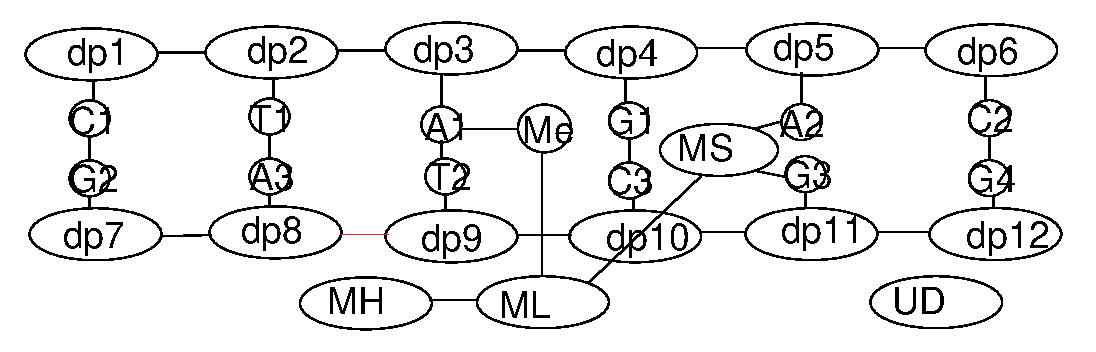
\includegraphics[width=1.0\textwidth]{mmr/state15}
  \caption[A six base pair DNA fragment.]{A six base pair DNA fragment, with a DNA mismatch and methylation of one strand. The proteins MutL, MutS, and  MutH are bonded to the strand and ready to recruit UvrD, which is not
  involved at this point yet.}
  \label{fig:state15}
\end{figure}

Next, $\MutH$ is ready to cleave the DNA at the right location. This is done by bonding to $\DP_8$ with the key 33 and, at the same time, breaking the bond between $\DP_8$ and $\DP_9$ (with the key 13). These two simultaneous reactions are represented by the following concerted actions transition.

\begin{flalign*}
&\xrightarrow{\{ws[33],\underline{p}[13]\}} (b_1[6];i_1).(a_1[24],m_1[40];r_1).A_1' \paral (b_6[9];i_6).(g_1[25];r_6).G_1' \paral  &&\\
&(b_2[7];i_2).(a_2[28],m_2;r_2).A_2' \paral (b_5[19];i_5).(t_2[24];r_5).T_2' \paral (b_{12}[20];i_{12}).(c_3[25];r_{12}).C_3'  \paral&&\\
&(b_8[21];i_8).(g_3[29];r_8).G_3' \paral ((p3_8[12],\bm{p5_8};\bm{s_8[33]}) \paral (b_8[18],d_8)).DP_8' \paral &&\\
&((\bm{p3_9},p5_9[14];s_9) \paral (b_9[19],d_9)).DP_9' \paral ((p3_{10}[14],p5_{10}[15];s_{10}) \paral (b_{10}[20],d_{10})).DP_{10}' \paral  &&\\
&((p3_{11}[15],p5_{11}[16];s_{11}) \paral (b_{11}[21],d_{11})).DP_{11}' \paral ((p3_{12}[16],p5_{12};s_{12}) \paral (b_{12}[22],d_{12})).DP_{12}' \paral  &&\\
&(m[40]).(n[31]).Me'\paral (k[28],k[29]).(l[30]).MutS' \paral (l[30]).(n[31]).(o[32]).MutL' \paral &&\\
&(o[32]).(\bm{w[33]}).MutH' \paral ((u;r) \paral (v;s)).UvrD'&&
\end{flalign*}
Next, {\em promotion} happens, which moves the bond with the key 33 from a weak action $s_8$ to a strong action $p5_8$ in one of the sites of $\DP_8$:
\begin{flalign*}
&\overset{ \rulename{prom}}\Rightarrow (b_1[6];i_1).(a_1[24],m_1[40];r_1).A_1' \paral (b_6[9];i_6).(g_1[25];r_6).G_1' \paral  &&\\
&(b_2[7];i_2).(a_2[28],m_2;r_2).A_2' \paral (b_5[19];i_5).(t_2[24];r_5).T_2' \paral (b_{12}[20];i_{12}).(c_3[25];r_{10}).C_3'  \paral &&\\
&(b_8[21];i_8).(g_3[29];r_8).G_3' \paral ((p3_8[12],\bm{p5_8[33]};\bm{s_8}) \paral (b_8[18],d_8)).DP_8' \paral &&\\
&((p3_9,\Red{\bm{p5_9[14]}};s_9) \paral (b_9[19],d_9)).DP_9' \paral ((\Red{\bm{p3_{10}[14]}},p5_{10}[15];\Blue{\bm{s_{10}}}) \paral (b_{10}[20],d_{10})).DP_{10}' \paral  &&\\
&((p3_{11}[15],p5_{11}[16];s_{11}) \paral (b_{11}[21],d_{11})).DP_{11}' \paral ((p3_{12}[16],p5_{12};s_{12}) \paral (b_{12}[22],d_{12})).DP_{12}' \paral  &&\\
&(m[40]).(n[31]).Me'\paral (k[28],k[29]).(l[30]).MutS' \paral (l[30]).(n[31]).(o[32]).MutL' \paral &&\\
&(o[32]).({w[33]}).MutH' \paral ((u;r) \paral (\Blue{\bm{v}};s)).UvrD'&&
\end{flalign*}
Note that $\MutH$ bonding with $\DP_8$ on $s_8$ (key 33) leads to breaking the bond between two deoxyribose/phosphate groups $\DP_8$ and $\DP_9$ (key13). 
%
%Note that execution of $s_8$ on $\DP_8$ leads to breaking a bond between two deoxyribose/phosphate groups. Specifically, bond 33 from $\MutH$ to $DP_8$ via actions $w$ and $s$ is formed and bond 13 between $p5$ in $\DP_8$ and $p3$ in  $\DP_9$ is broken. %We use concerted actions and rewriting for this.
%
The situation after this step is shown in Figure~\ref{fig:state2}, where the new bond (key 33) is shown as a blue line. The broken bond (key 13) is indicated by a red dotted line, and henceforth, we shall use this representation for broken bonds. Such dotted lines will be left out in subsequent figures to indicate that the relevant bonds no longer exist.  This has now the right DNA strand cleaved.

\begin{figure}[h!]
\psfrag{13}[cc][][0.8][0]{$13$}
\psfrag{33}[cc][][0.8][0]{$33$}
\psfrag{dp1}{$DP_1$}
\psfrag{dp2}{$DP_2$}
\psfrag{dp3}{$DP_3$}
\psfrag{dp4}{$DP_4$}
\psfrag{dp5}{$DP_5$}
\psfrag{dp6}{$DP_6$}
\psfrag{dp7}{$DP_7$}
\psfrag{dp8}{$DP_8$}
\psfrag{dp9}{$DP_9$}
\psfrag{dp10}{$DP_{10}$}
\psfrag{dp11}{$DP_{11}$}
\psfrag{dp12}{$DP_{12}$}
\psfrag{A1}[cc][][0.8][0]{$A_1$}
\psfrag{A2}[cc][][0.8][0]{$A_2$}
\psfrag{A3}[cc][][0.8][0]{$A_3$}
\psfrag{T1}[cc][][0.8][0]{$T_1$}
\psfrag{T2}[cc][][0.8][0]{$T_2$}
\psfrag{C1}[cc][][0.8][0]{$C_1$}
\psfrag{C2}[cc][][0.8][0]{$C_2$}
\psfrag{C3}[cc][][0.8][0]{$C_3$}
\psfrag{G1}[cc][][0.8][0]{$G_1$}
\psfrag{G2}[cc][][0.8][0]{$G_2$}
\psfrag{G3}[cc][][0.8][0]{$G_3$}
\psfrag{G4}[cc][][0.8][0]{$G_4$}
\psfrag{Me}{${\mathit{Me}}$}
\psfrag{MS}{${\mathit{MutS}}$}
\psfrag{ML}{${\mathit{MutL}}$}
\psfrag{MH}{${\mathit{MutH}}$}
\psfrag{UD}{${\mathit{UvrD}}$}
  \centering
    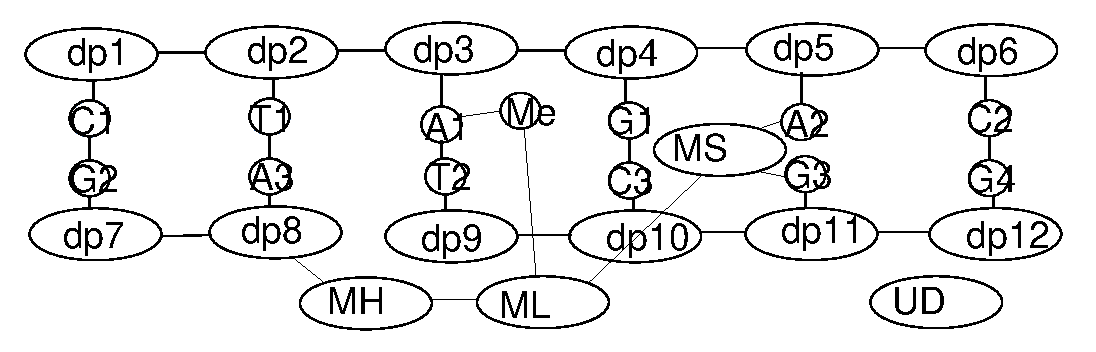
\includegraphics[width=1.0\textwidth]{mmr/state2}
  \caption[A six base pair DNA fragment.]{%A six base pair DNA fragment, with a DNA mismatch and methylation of one strand.
  The mismatch has been detected by $\MutS$, and $\MutH$ and $\MutL$ have been recruited. $\MutL$ has detected the methylation, and $\MutH$ has cleaved the strand containing the wrong base by bonding to $DP_8$ (blue line) and thus breaking   the bond between $DP_8$ and $DP_9$ (red dotted line).}
  \label{fig:state2}
\end{figure}

Next, the protein $\UvrD$ gets involved in the repair. It uses the cleavage to remove pairs of deoxyribose/phosphate groups and bases.
Firstly, $\UvrD$ bonds to $\DP_{10}$ (key 34) and thus breaks the bond between $\DP_{10}$ and its left neighbour
$\DP_9$ (key 14). Then the bond 34 is promoted from weak action $s_{10}$ to strong action $p3_{10}$:

\begin{flalign*}
&\xrightarrow{\{sv[34],\underline{p}[14]\}}  \overset{ \rulename{prom}}\Rightarrow  
(b_1[6];i_1).(\Red{\bm{a_1[24]}},m_1[40];r_1).A_1' \paral  (b_6[9];i_6).(g_1[25];r_6).G_1' \paral &&\\
&(b_2[7];i_2).(a_2[28],m_2;r_2).A_2' \paral (b_5[19];i_5).(\Red{\bm{t_2[24]}};\Blue{\bm{r_5}}).T_2' \paral (b_{12}[20];i_{12}).(c_3[25];r_{12}).C_3'  \paral&&\\
&(b_8[21];i_8).(g_3[29];r_8).G_3' \paral ((p3_8[12],p5_8[33];s_8) \paral (b_8[18],d_8)).\DP_8' \paral &&\\
&((p3_9,\bm{p5_9};s_9) \paral (b_9[19],d_9)).\DP_9' \paral ((\bm{p3_{10}[34]},p5_{10}[15];\bm{s_{10}}) \paral (b_{10}[20],d_{10})).\DP_{10}' \paral  &&\\
&((p3_{11}[15],p5_{11}[16];s_{11}) \paral (b_{11}[21],d_{11})).\DP_{11}' \paral ((p3_{12}[16],p5_{12};s_{12}) \paral (b_{12}[22],d_{12})).\DP_{12}' \paral  &&\\
&(m[40]).(n[31]).\Me'\paral (k[28],k[29]).(l[30]).\MutS' \paral (l[30]).(n[31]).(o[32]).\MutL' \paral &&\\
&(o[32]).(w[33]).\MutH' \paral ((\Blue{\bm{u}};r) \paral (\bm{v[34]};s)).\UvrD'&&
\end{flalign*}

Secondly, $\UvrD$ combines with $T_2$ (key 35) thus breaking the bond between $T_2$ and its paired base $A_1$ (key 24). This concerted actions transition is followed immediately by an application of \rulename{prom}, which moves a bond from weak action $r_5$ to strong actions $t_2$.
%These concerted actions transitions and applications of \rulename{prom} are as follows:

\begin{flalign*}
&\xrightarrow{\{ur[35],\underline{at}[24]\}}  \overset{ \rulename{prom}}\Rightarrow 
(b_1[6];i_1).(\bm{a_1},m_1[40];r_1).A_1' \paral  (b_6[9];i_6).(g_1[25];r_6).G_1' \paral &&\\
&(b_2[7];i_2).(a_2[28],m_2;r_2).A_2' \paral (b_5[19];i_5).(\bm{t_2[35]};\bm{r_5}).T_2' \paral (b_{12}[20];i_{12}).(c_3[25];r_{12}).C_3'  \paral&&\\
&(b_8[21];i_8).(g_3[29];r_8).G_3' \paral ((p3_8[12],p5_8[33];s_8) \paral (b_8[18],d_8)).\DP_8' \paral &&\\
&((p3_9,p5_9;s_9) \paral (b_9[19],d_9)).\DP_9' \paral ((p3_{10}[34],p5_{10}[15];\bm{s_{10}}) \paral (b_{10}[20],d_{10})).\DP_{10}' \paral  &&\\
&((p3_{11}[15],p5_{11}[16];s_{11}) \paral (b_{11}[21],d_{11})).\DP_{11}' \paral ((p3_{12}[16],p5_{12};s_{12}) \paral (b_{12}[22],d_{12})).\DP_{12}' \paral  &&\\
&(m[40]).(n[31]).\Me'\paral (k[28],k[29]).(l[30]).\MutS' \paral (l[30]).(n[31]).(o[32]).\MutL' \paral &&\\
&(o[32]).(w[33]).\MutH' \paral ((\bm{u[35]};r) \paral (v[34];s)).\UvrD'&&
\end{flalign*}
Note that $\UvrD$ does not attach to $\DP_9$ initially, but to $\DP_{10}$. If it had been attached to $\DP_9$, it would have had no connection to the DNA strand once the bonds of $DP_9$ and $T_2$ to the rest of DNA strand have been broken.

The removal of the first base and deoxyribose/phosphate group is shown in Figure~\ref{fig:state3}. The
blue lines show the bonds that have been created and the red dotted lines indicate the bonds that have been broken.
% and formed during concerted actions.
The two pairs of concerted actions transitions have the keys (34,14) and (35,24) respectively.

\begin{figure}[h!]
\psfrag{24}[cc][][0.8][0]{$24$}
\psfrag{14}[cc][][0.8][0]{$14$}
\psfrag{35}[cc][][0.8][0]{$35$}
\psfrag{34}[cc][][0.8][0]{$34$}
\psfrag{dp1}{${DP_1}$}
\psfrag{dp2}{${DP_2}$}
\psfrag{dp3}{${DP_3}$}
\psfrag{dp4}{${DP_4}$}
\psfrag{dp5}{${DP_5}$}
\psfrag{dp6}{${DP_6}$}
\psfrag{dp7}{${DP_7}$}
\psfrag{dp8}{${DP_8}$}
\psfrag{dp9}{${DP_9}$}
\psfrag{dp10}{${DP_{10}}$}
\psfrag{dp11}{${DP_{11}}$}
\psfrag{dp12}{${DP_{12}}$}
\psfrag{A1}[cc][][0.8][0]{${A_1}$}
\psfrag{A2}[cc][][0.8][0]{${A_2}$}
\psfrag{A3}[cc][][0.8][0]{${A_3}$}
\psfrag{T1}[cc][][0.8][0]{${T_1}$}
\psfrag{T2}[cc][][0.8][0]{${T_2}$}
\psfrag{C1}[cc][][0.8][0]{${C_1}$}
\psfrag{C2}[cc][][0.8][0]{${C_2}$}
\psfrag{C3}[cc][][0.8][0]{${C_3}$}
\psfrag{G1}[cc][][0.8][0]{${G_1}$}
\psfrag{G2}[cc][][0.8][0]{${G_2}$}
\psfrag{G3}[cc][][0.8][0]{${G_3}$}
\psfrag{G4}[cc][][0.8][0]{${G_4}$}
\psfrag{Me}{${\mathit{Me}}$}
\psfrag{MS}{${\mathit{MutS}}$}
\psfrag{ML}{${\mathit{MutL}}$}
\psfrag{MH}{${\mathit{MutH}}$}
\psfrag{UD}{${\mathit{UvrD}}$}
  \centering
    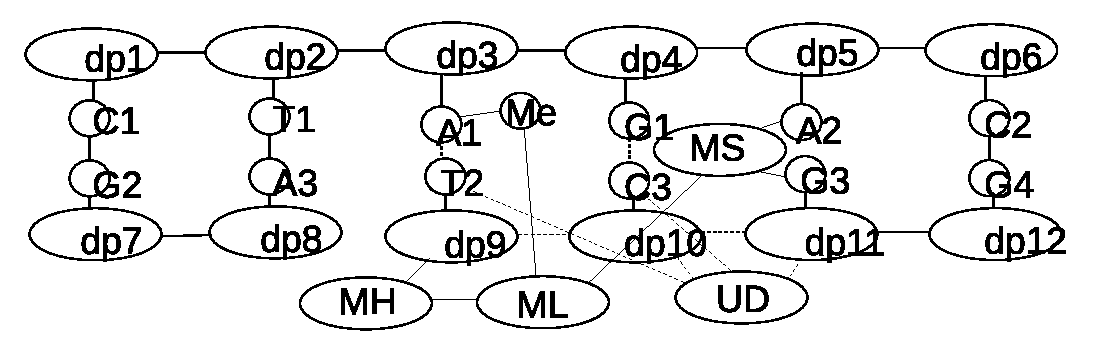
\includegraphics[width=1.0\textwidth]{mmr/state3}
  \caption[A six base pair DNA fragment.]{%A six base pair DNA fragment, with a DNA mismatch and methylation of one strand.
  $\UvrD$ has now bonded to $T_2$ and $\DP_{10}$ (blue lines), breaking the bonds of those molecules to the rest of the DNA (red dotted lines). %In a next step, $\UvrD$ can now ``walk'' along the DNA strand, and remove the next pair of $\DP$ and base molecules.
}
  \label{fig:state3}
\end{figure}

$\UvrD$ can now ``walk'' along the lower chain of the strand towards the right end.
%As opposed to BER, the bonds between the base pairs are now broken during the walk.
Concurrently, the bonds between the deoxyribose/phosphate groups are also broken as $\UvrD$ progresses. We write these reactions as two separate concerted actions transitions for clarity, with the first transition in full,  and note that this is the first time we have used the new \rulename{concert3} SOS rule.
\begin{flalign*}
& (b_1[6];i_1).(a_1,m_1[40];r_1).A_1' \paral  (b_6[9];i_6).(g_1[25];r_6).G_1' \paral &&\\
&(b_2[7];i_2).(a_2[28],m_2;r_2).A_2' \paral (b_5[19];i_5).(t_2[35]; r_5).T_2' \paral (b_{12}[20];i_{12}).(c_3[25];r_{12}).C_3'  \paral&&\\
&(b_8[21];i_8).(g_3[29];r_8).G_3' \paral ((p3_8[12],p5_8[33];s_8) \paral (b_8[18],d_8)).\DP_8' \paral &&\\
&((p3_9,p5_9;s_9) \paral (b_9[19],d_9)).\DP_9' \paral ((\Red{\bm{p3_{10}[34]}},\Red{\bm{p5_{10}[15]}};s_{10}) 
 \paral (b_{10}[20],d_{10})).\DP_{10}' \paral  &&\\
&((\Red{\bm{p3_{11}[15]}},p5_{11}[16];\Blue{\bm{s_{11}}}) \paral (b_{11}[21],d_{11})).\DP_{11}' \paral ((p3_{12}[16],p5_{12};s_{12}) \paral (b_{12}[22],d_{12})).\DP_{12}' \paral  &&\\
&(m[40]).(n[31]).\Me'\paral (k[28],k[29]).(l[30]).\MutS' \paral (l[30]).(n[31]).(o[32]).\MutL' \paral &&\\
&(o[32]).(w[33]).\MutH' \paral ((u[35];r) \paral (\Red{\bm{v[34]}};\Blue{\bm{s}})).\UvrD'&&\\
&\xrightarrow{\{ss[36],\underline{vp3}[34],\underline{p}[15]\}}
\overset{ \rulename{prom}}\Rightarrow \; \overset{ \rulename{prom}}\Rightarrow\\
& (b_1[6];i_1).(a_1,m_1[40];r).A_1' \paral (b_6[9];i_6).(\Red{\bm{g_1[25]}};r_3).G_1' \paral &&\\
&(b_2[7];i_2).(a_2[28],m_2;r).A_2' \paral (b_5[19];i_5).(\Red{\bm{t_2[35]}};r_2).T_2' \paral (b_{11}[20];i_{11}).(\Red{\bm{c_3[25]}};\Blue{\bm{r_8}}).C_3'  \paral&&\\
&(b_8[21];i_8).(g_2[29];r_4).G_3' \paral ((p3_8[12],p5_8[33];s_8) \paral (b_8[18],d_8)).\DP_8' \paral &&\\
&((p3_9,p5_9;s_9) \paral (b_9[19],d_9)).\DP_9' \paral ((\bm{p3_{10},p5_{10}};s_{10}) \paral (b_{10}[20],d_{10})).\DP_{10}' \paral &&\\
&((\bm{p3_{11}[36]},p5_{11}[16];\bm{s_{11}}) \paral (b_{11}[21],d_{11})).\DP_{11}' \paral ((p3_{12}[16],p5_{12};s_{12}) \paral (b_{12}[22],d_{12})).\DP_{12}' \paral  &&\\
&(m[40]).(n[31]).\Me'\paral (k[28],k[29]).(l[30]).\MutS' \paral (l[30]).(n[31]).(o[32]).\MutL' \paral &&\\
&(o[32]).(w[33]).\MutH' \paral ((\Red{\bm{u[35]}};\Blue{\bm{r}}) \paral (\bm{v[36]};\bm{s})).\UvrD'&&
\end{flalign*}
Notice that promotion has moved a bond from $s_{11}$ to $p3_{11}$ and from $s$ to $v$. 

Next,  $\UvrD$ combines with $C_3$ thus breaking bonds with keys 35 and 25:
\begin{flalign*}
&\xrightarrow{\{rr[37],\underline{tu}[35],\underline{cg}[25]\}}
\overset{ \rulename{prom}}\Rightarrow \; \overset{ \rulename{prom}}\Rightarrow
 (b_1[6];i_1).(a_1,m_1[40];r).A_1' \paral (b_6[9];i_6).(\bm{g_1};r_3).G_1' \paral  &&\\
&(b_2[7];i_2).(a_2[28],m_2;r).A_2' \paral (b_5[19];i_5).(\bm{t_2};r_2).T_2' \paral (b_{11}[20];i_{11}).(\bm{c_3[37]};\bm{r_8}).C_3'  \paral&&\\
&(b_8[21];i_8).(g_2[29];r_4).G_3' \paral  ((p3_8[12],p5_8[33];s_8) \paral (b_8[18],d_8)).\DP_8' \paral &&\\
&((p3_9,p5_9;s_9) \paral (b_9[19],d_9)).\DP_9' \paral ((p3_{10},p5_{10};s_{10}) \paral (b_{10}[20],d_{10})).\DP_{10}' \paral &&\\
&((p3_{11}[36],p5_{11}[16];s_{11}) \paral (b_{11}[21],d_{11})).\DP_{11}' \paral ((p3_{12}[16],p5_{12};s_{12}) \paral (b_{12}[22],d_{12})).\DP_{12}' \paral  &&\\
&(m[40]).(n[31]).\Me'\paral (k[28],k[29]).(l[30]).\MutS' \paral (l[30]).(n[31]).(o[32]).\MutL' \paral &&\\
&(o[32]).(w[33]).\MutH' \paral ((\bm{u[37]};\bm{r}) \paral (v[36];s)).\UvrD'&&
\end{flalign*}
Promotion moves bonds from
$r_8$ to $c_3$ and from $r$ to $u$ below.


The resulting system is shown in Figure~\ref{fig:state4}. Here, the first  base $T_2$ and deoxyribose/phosphate group
$\DP_9$ have been removed (shown in grey) and $\UvrD$ has moved to the next  base $C_3$
and deoxyribose/phosphate group $\DP_{10}$, again to remove them. The two concerted actions transitions that represent these reactions are with the keys (36,34,15) and (37,35,25) respectively.
%Notice that here we have used the new rule \rulename{concert 3}.

\begin{figure}[h!]
\psfrag{25}[cc][][0.8][0]{$25$}
\psfrag{15}[cc][][0.8][0]{$15$}
\psfrag{35}[cc][][0.8][0]{$35$}
\psfrag{34}[cc][][0.8][0]{$34$}
\psfrag{36}[cc][][0.8][0]{$36$}
\psfrag{37}[cc][][0.8][0]{$37$}
\psfrag{dp1}{${DP_1}$}
\psfrag{dp2}{${DP_2}$}
\psfrag{dp3}{${DP_3}$}
\psfrag{dp4}{${DP_4}$}
\psfrag{dp5}{${DP_5}$}
\psfrag{dp6}{${DP_6}$}
\psfrag{dp7}{${DP_7}$}
\psfrag{dp8}{${DP_8}$}
\psfrag{dp9}{\color{gray}${DP_9}$}
\psfrag{dp10}{${DP_{10}}$}
\psfrag{dp11}{${DP_{11}}$}
\psfrag{dp12}{${DP_{12}}$}
\psfrag{A1}[cc][][0.8][0]{${A_1}$}
\psfrag{A2}[cc][][0.8][0]{${A_2}$}
\psfrag{A3}[cc][][0.8][0]{${A_3}$}
\psfrag{T1}[cc][][0.8][0]{${T_1}$}
\psfrag{T2}[cc][][0.8][0]{\color{gray}${T_2}$}
\psfrag{C1}[cc][][0.8][0]{${C_1}$}
\psfrag{C2}[cc][][0.8][0]{${C_2}$}
\psfrag{C3}[cc][][0.8][0]{${C_3}$}
\psfrag{G1}[cc][][0.8][0]{${G_1}$}
\psfrag{G2}[cc][][0.8][0]{${G_2}$}
\psfrag{G3}[cc][][0.8][0]{${G_3}$}
\psfrag{G4}[cc][][0.8][0]{${G_4}$}
\psfrag{Me}{${\mathit{Me}}$}
\psfrag{MS}{${\mathit{MutS}}$}
\psfrag{ML}{${\mathit{MutL}}$}
\psfrag{MH}{${\mathit{MutH}}$}
\psfrag{UD}{${\mathit{UvrD}}$}
  \centering
    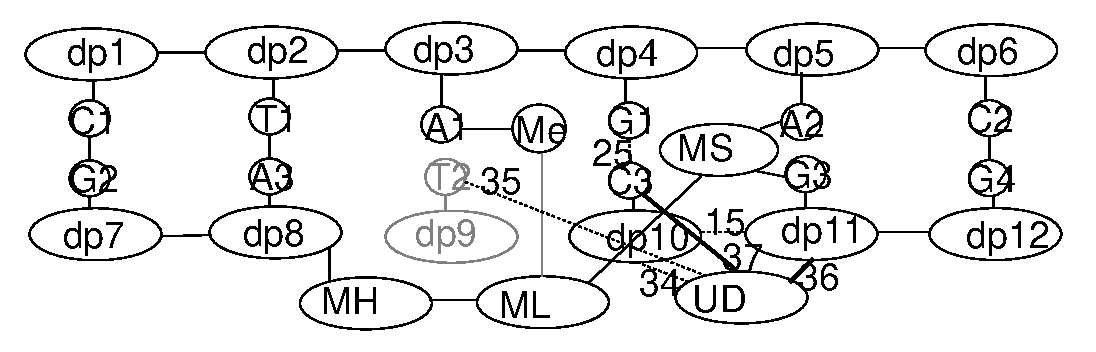
\includegraphics[width=1.0\textwidth]{mmr/state4}
  \caption[A six base pair DNA fragment.]{%A six base pair DNA fragment, with a DNA mismatch and methylation of one strand.
  $\UvrD$ has now bonded to $C_3$ and $\DP_{11}$ (bonds shows as blue lines), breaking the bonds of those molecules to the rest of the DNA via concerted actions (shown as red dotted lines). The group of $T_2$ and $\DP_{9}$ is no longer attached to the DNA (shown in grey). % This process can continue for more pairs.
}
  \label{fig:state4}
\end{figure}

This process continues until the offending base $G_3$ has been removed. We do not show concerted actions transitions that model this since they correspond very closely to the last two transitions. Figure~\ref{fig:state6} shows the result of these two transitions which remove of the offending base.
%We do not model how the number of base pairs to remove is determined.
%In reality, that number is not fixed, but is determined by the interal workings of the protein, where the number is statistically distributed.
Once this is done and the MutH, MutL, and MutS proteins have detached we get the situation shown in Figure~\ref{fig:state7}.


\begin{figure}[t!]
\psfrag{29}[cc][][0.8][0]{$29$}
\psfrag{16}[cc][][0.8][0]{$16$}
\psfrag{38}[cc][][0.8][0]{$38$}
\psfrag{39}[cc][][0.8][0]{$39$}
\psfrag{36}[cc][][0.8][0]{$36$}
\psfrag{37}[cc][][0.8][0]{$37$}
\psfrag{dp1}{${DP_1}$}
\psfrag{dp2}{${DP_2}$}
\psfrag{dp3}{${DP_3}$}
\psfrag{dp4}{${DP_4}$}
\psfrag{dp5}{${DP_5}$}
\psfrag{dp6}{${DP_6}$}
\psfrag{dp7}{${DP_7}$}
\psfrag{dp8}{${DP_8}$}
\psfrag{dp9}{${DP_9}$}
\psfrag{dp10}{\color{gray}${DP_{10}}$}
\psfrag{dp11}{${DP_{11}}$}
\psfrag{dp12}{${DP_{12}}$}
\psfrag{A1}[cc][][0.8][0]{${A_1}$}
\psfrag{A2}[cc][][0.8][0]{${A_2}$}
\psfrag{A3}[cc][][0.8][0]{${A_3}$}
\psfrag{T1}[cc][][0.8][0]{${T_1}$}
\psfrag{T2}[cc][][0.8][0]{${T_2}$}
\psfrag{C1}[cc][][0.8][0]{${C_1}$}
\psfrag{C2}[cc][][0.8][0]{${C_2}$}
\psfrag{C3}[cc][][0.8][0]{\color{gray}${C_3}$}
\psfrag{G1}[cc][][0.8][0]{${G_1}$}
\psfrag{G2}[cc][][0.8][0]{${G_2}$}
\psfrag{G3}[cc][][0.8][0]{${G_3}$}
\psfrag{G4}[cc][][0.8][0]{${G_4}$}
\psfrag{Me}{${\mathit{Me}}$}
\psfrag{MS}{${\mathit{MutS}}$}
\psfrag{ML}{${\mathit{MutL}}$}
\psfrag{MH}{${\mathit{MutH}}$}
\psfrag{UD}{${\mathit{UvrD}}$}
  \centering
    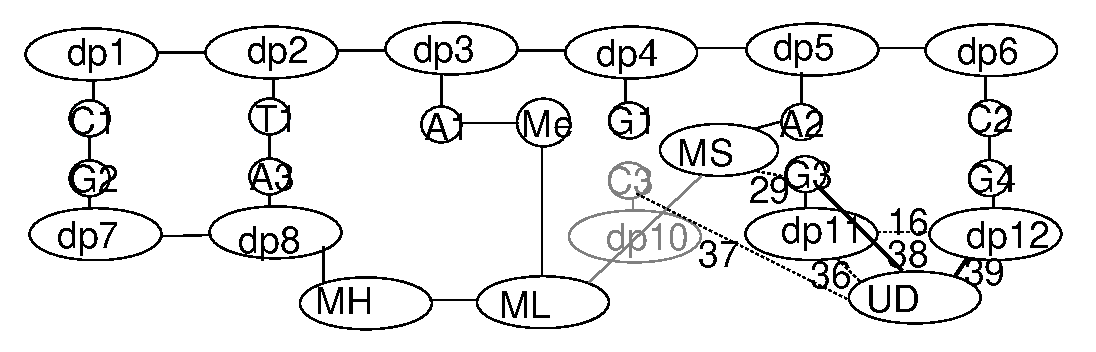
\includegraphics[width=1.0\textwidth]{mmr/state6}
  \caption[A six base pair DNA fragment.]{%A six base pair DNA fragment, with a DNA mismatch and methylation of one strand.
$\UvrD$ has now bonded to $G_3$ (the offending base) and $\DP_{12}$, breaking the bonds of those molecules to the rest of the DNA via concerted actions. The $G_3$-$\DP_{10}$ group, containing the offending base $G_3$,  is now removed (shown in grey).}
  \label{fig:state6}
\end{figure}

\begin{figure}[]
\psfrag{dp1}{${DP_1}$}
\psfrag{dp2}{${DP_2}$}
\psfrag{dp3}{${DP_3}$}
\psfrag{dp4}{${DP_4}$}
\psfrag{dp5}{${DP_5}$}
\psfrag{dp6}{${DP_6}$}
\psfrag{dp7}{${DP_7}$}
\psfrag{dp8}{${DP_8}$}
\psfrag{dp9}{${DP_9}$}
\psfrag{dp10}{${DP_{10}}$}
\psfrag{dp11}{${DP_{11}}$}
\psfrag{dp12}{${DP_{12}}$}
\psfrag{A1}[cc][][0.8][0]{${A_1}$}
\psfrag{A2}[cc][][0.8][0]{${A_2}$}
\psfrag{A3}[cc][][0.8][0]{${A_3}$}
\psfrag{T1}[cc][][0.8][0]{${T_1}$}
\psfrag{T2}[cc][][0.8][0]{${T_2}$}
\psfrag{C1}[cc][][0.8][0]{${C_1}$}
\psfrag{C2}[cc][][0.8][0]{${C_2}$}
\psfrag{C3}[cc][][0.8][0]{${C_3}$}
\psfrag{G1}[cc][][0.8][0]{${G_1}$}
\psfrag{G2}[cc][][0.8][0]{${G_2}$}
\psfrag{G3}[cc][][0.8][0]{${G_3}$}
\psfrag{G4}[cc][][0.8][0]{${G_4}$}
\psfrag{Me}{${\mathit{Me}}$}
\psfrag{MS}{${\mathit{MutS}}$}
\psfrag{ML}{${\mathit{MutL}}$}
\psfrag{MH}{${\mathit{MutH}}$}
\psfrag{UD}{${\mathit{UvrD}}$}
  \centering
    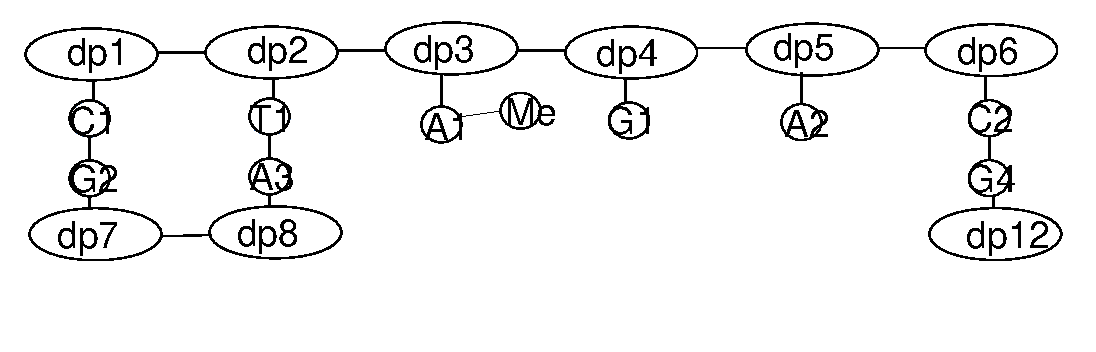
\includegraphics[width=1.0\textwidth]{mmr/state7}\vspace{-1cm}
  \caption[A six base pair DNA fragment.]{A DNA fragment with a gap of three bases in one strand produced by MMR.}
  \label{fig:state7}
\end{figure}
The resulting system is now ready for other proteins to replace the bases and deoxyribose/phosphate groups. Notice that the remaining strand contains the necessary information for this, in particular that only a $T$ base can bond with $A_1$ and $A_2$ and that a $C$ must bond with $G_1$. Note that the methyl group stays attached to $A_1$, since it is still an old DNA strand. Also the appropriate groups in the new, lower half will be methylated, so that both strands are marked as old material after the next DNA duplication process.

Our modelling has not considered any aspects of spatial configuration of proteins and bases. As in the BER example,
this means that UvrD could bond to any deoxyribose/phosphate group, not just the neighbouring one. It also means that we have not modelled the formation of the loop in the DNA, which is crucial for cleaving the correct strand.


